%%% In this section, you will describe all of the various artifacts that you will generate and maintain during the project life cycle. Describe the purpose of each item below, how the content will be generated, where it will be stored, how often it will be updated, etc. Replace the default text for each section with your own description. Reword this paragraph as appropriate.

\subsection{Major Documentation Deliverables}

\subsubsection{Project Charter}
\begin{itemize}
  \item Will be maintained under both version control in a git repository and as a word document.
  \item Will be updated whenever an important aspect (such as implementation, architecture, ideas, etc.) is changed.
  \item The initial version will be submitted when the first sprint is due (October 23rd).
  \item The final version will be submitted whenever the final submission of the project is.
\end{itemize}

\subsubsection{System Requirements Specification}
\begin{itemize}
  \item Will be maintained under both version control in a git repository and as a word document.
  \item Will be updated whenever an important aspect (such as system requirements) is changed.
  \item The initial version will be submitted whenever it is first due.
  \item The final version will be submitted whenever the final submission of the project is.
\end{itemize}

\subsubsection{Architectural Design Specification}
\begin{itemize}
  \item Will be maintained under both version control in a git repository and as a word document.
  \item Will be updated whenever an important aspect (such as the underlying architecture) is changed.
  \item The initial version will be submitted whenever it is first due.
  \item The final version will be submitted whenever the final submission of the project is.
\end{itemize}

\subsubsection{Detailed Design Specification}
\begin{itemize}
  \item Will be maintained under both version control in a git repository and as a word document.
  \item Will be updated whenever an important aspect (such as the design system) is changed.
  \item The initial version will be submitted whenever it is first due.
  \item The final version will be submitted whenever the final submission of the project is.
\end{itemize}

\subsection{Recurring Sprint Items}
\subsubsection{Product Backlog}
\begin{itemize}
  \item Items will be added by order of prioritization. The items will be prioritized by whether or not they are required for the core of the product to work.
  \item A group vote will be administered to determine how a task is prioritized. Someone in the group is allowed to take care of it sooner than its determined priority if they have the time for it.
  \item GitHub offers a kanban-style board for projects, so we will be utilize this to keep track of the product backlog.
\end{itemize}

\subsubsection{Sprint Planning}
\begin{itemize}
  \item The team will meet up and discuss the requirements that need to be finished, and the tasks that are on the project board, and align them with the sprint intervals in the Senior Design course.
  \item There will be 8 sprints total. (4 in SD I, and 4 in SD II).
\end{itemize}

\subsubsection{Sprint Goal}
\begin{itemize}
  \item The group leader and stakeholder will decide the sprint goal once the team has determined what needs to be accomplished in said sprint.
\end{itemize}

\subsubsection{Sprint Backlog}
\begin{itemize}
  \item The team as a whole will decide what items make their way into the backlog.
  \item GitHub offers a kanban-style board for projects, so we will be utilize this to keep track of the product backlog.
\end{itemize}

\subsubsection{Task Breakdown}
\begin{itemize}
  \item Individual tasks will be assigned based off of skill level, willingness to learn subject material, or if anyone voluntarily claims said task.
  \item Team members will post updates to assigned tasks using GitHub Issues & Pull Requests.
\end{itemize}

\subsubsection{Sprint Burn Down Charts}
\begin{itemize}
  \item Responsibility of the burndown chart for each sprint will be decided on either a team member taking the initiative, or from whoever has yet to take responsibility for it.
\end{itemize}

\begin{figure}[h!]
    \centering
    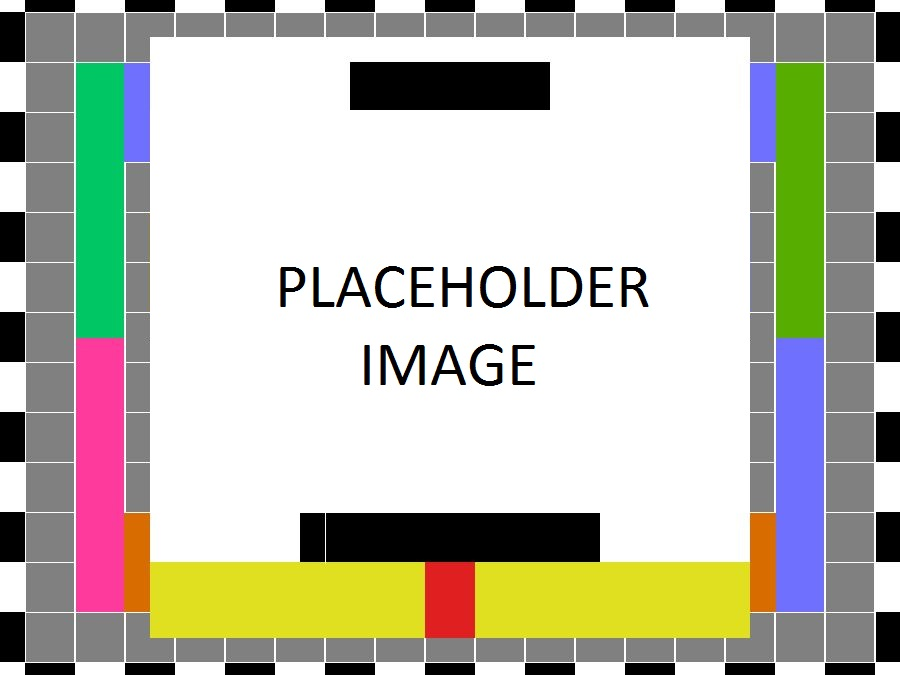
\includegraphics[width=0.5\textwidth]{images/test_image}
    \caption{Example sprint burn down chart}
\end{figure}

\subsubsection{Sprint Retrospective}
\begin{itemize}
  \item After the completion of each sprint, the team will meet, discuss, and take notes of the retrospective.
  \item Topics that will be documented include tasks completed, tasks not completed, risks, implementation issues, personal challenges, etc.
  \item The retrospective will be submitted shortly after the sprint is completed.
\end{itemize}

\subsubsection{Individual Status Reports}
\begin{itemize}
  \item Statuses that should be reported by each individual team member includes personal issues that give risks to completing the work, challenges faced & lack of understanding in assigned tasks, new implementation ideas, and anything else they see fit to note.
\end{itemize}

\subsubsection{Engineering Notebooks}
\begin{itemize}
  \item Each member will “witness” one other member’s notebook during a meeting. A minimum one page will be completed per interval. Each member must be at a meeting to get their ENB witnessed.
  \item An individual’s notebook will need to be updated every two weeks with meeting notes and ideas.
\end{itemize}

\subsection{Closeout Materials}
\begin{itemize}
  \item N/A
\end{itemize}

\subsubsection{System Prototype}
\begin{itemize}
  \item The final system prototype will include the website for aggregating all the music playlists. It will be demonstrated on May 1st, 2019.
\end{itemize}

\subsubsection{Project Poster}
\begin{itemize}
  \item The project poster will include screenshots of the final project being developed, why we created the project and how to use the project.
\end{itemize}

\subsubsection{Web Page}
\begin{itemize}
  \item The project web page will have a link to download the service on it and will explain the service. It will be accessible to the public and will be delivered by May 1st, 2019.
\end{itemize}

\subsubsection{Demo Video}
\begin{itemize}
  \item The demo video will show the user how to sign in to the providers, link their streaming playlists to their current session, and choose music from each playlists from the providers that are aggregated together.
\end{itemize}

\subsubsection{Source Code}
\begin{itemize}
  \item We will maintain our source code by hosting our code base on GitHub. We will adopt Git as our source control. A website will be the source of the product.
\end{itemize}

\subsubsection{Source Code Documentation}
\begin{itemize}
  \item We will use React Docgen for creating documentation (https://github.com/reactjs/react-docgen). Which can be extracted as a json blob.
\end{itemize}

\subsubsection{Hardware Schematics}
\begin{itemize}
  \item N/A (There will be no hardware for this project)
\end{itemize}

\subsubsection{CAD files}
\begin{itemize}
  \item N/A (There will be no hardware in this project. Therefore, there will not be a need for CAD files.)
\end{itemize}

\subsubsection{Installation Scripts}
\begin{itemize}
  \item A project README and installation steps will be provided in the project repo.
\end{itemize}

\subsubsection{User Manual}
\begin{itemize}
  \item A project README and installation steps will be provided in the project repo.
\end{itemize}
